\chapter{Synchronizing the clients}

The synchronization of the animations have two major steps. First of all we have a continously running animation that takes input from the Tween class. This animation could be synchronized by giving every client a notion of how much delay there is between that client and a master, a master that could be the server.

The second step where to adapt the time the clients played specific parts of the animation when recieving a render event message from the server. Here we also faced the challange that one client could have a latency bigger than we could accept so that we would have to adjust this client some other way. A solution for this was implemented using frameskipping. 

\section{Synchronizing the time}

Because the clients may run on different computers the computer clock time cannot be used as a parameter to the animations since the computer clocks are unlikely to be in sync with each other. As shown in chapter 1 this is a well known problem in distributed systems, so the first step would be to implement one or several existing synchronization algorithms. 

A combination of the Berkley algoritm (ref section) and NTP (ref section) was used to synchronize the time of the clients and the server. Both NTP and the Berkley algorithm are designed to be used in intranets since they assume an evenly distributed delay. The end product that the work in this thesis is intended to be used in is assumed to run on an intranet. The accuracy given by these algoritms was assumed to be good enough. 

An artificial time is created both on the server and on the clients on start and this time never manipulated. Instead a delta value added to the artificial time is used as input to the animations.  

\subsection {Distributing deltas}

The server initiates the synchronization with the clients by sending a sync event message to the clients. The clients reply with the time they recieved the message, the time they send their reply and their old delta-value. The server then calculates each clients delta and sends each client a message containing their new delta. 

If the value of the old delta of the client and the new delta calculated by the server differs more than 2 milliseconds the server will send a new sync event as a message to the client, repeating the procedure until the delta is stable. 

Every time a new client connects to the server this client needs to synchronize its time with the server's. 

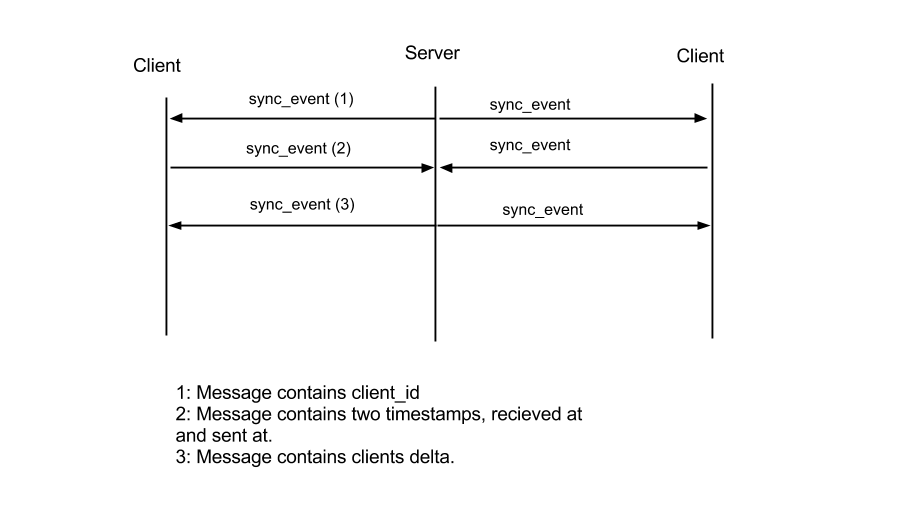
\includegraphics[width=1.0\textwidth]{figures/comm.png}

\subsection{Calculating deltas}
An implementation of NTP was used to calculate each clients latency, shown below.

\begin{verbatim}
self.delta = ((self.t_1 - self.t_0) + (self.t_2 - self.t_3))/2
\end{verbatim}

\subsection {Using the delta values}

All animations must take a timestamp as a parameter for playback. This is used to timestep through the animation. To create the timestamp the client uses the time acquired when the delta is added to its own local time. This way all client's animations will be synchronized, they will be at the same stage in the animation at the same time given that they have their correct delta value. 



\section{Distributing latencies}

\subsection{Finding the latency of a client}
The latency of each client is calculated by the server and sent to the client in an latency\_update\_event, along with the maximum latecy. The maximum latency is the latency of the client with the greatest latency. The client then calculates the wait period to sync to the client with the highest latency by subtracting its own latency from the maximum latency.

Client latencies are stored in an array on the server, everytime a client latency is updated the value of that respective row in the array is updated. The maximum latency is simply the largest number in this array.

Every time a new client connects to the server the server must send latency\_update\_events to all clients since the new connecting clients latency might be bigger than the current maximum latency. The maximum latency then needs to be redistributed to all clients. 

\begin{figure}[h!]
	\begin{displaymath}
		\text{applied\_latency} = \text{maximum\_latency} - \text{latency}
	\end{displaymath}
	\caption{Calculating the applied latency}
	\label{fig:applatency}
\end{figure} 

\subsection{Delaying animation start based on latency}
Before handling a new render event the client waits for the number of milliseconds specified by its applied latency. This way the faster clients will compensate for the slow ones. 

\subsection{Skipping frames if delay is to long}
If a clients latency is higher than a set threshold, the highest latency under the treshold is selected as the maximum latency and the client(s) above the threshold skip ahead instead. The clients that skip ahead will use their latency to skip that amount of time ahead in the animation. 



